\section{Cost function}\label{sec:cost_fkt}
\todotom{I think it is a good idea to treat the data below as if it were a prediction of the future prices.
W.r.t. the term 'cost function', I think it's a bit misplaced here. What you have in the graph is the cost-of-energy as a function of time. However, when you use the term 'cost function' it might be confused with the term 'objective function', which in your case will be the product between the cost-of-energy and the energy consumed.}


To minimize the running cost of the system a cost function of the electrical price is needed. Predicting future prices is an extensive task that depends on many factors e.g user consumption and weather conditions. Due to the fact that the learning goals of this project is not to derive a high precision predictive model that describe future electrical prices, data gathered from \cite{Electrical_price} is used instead. This data is used to represent the output of a high quality cost function, where 60 hours can be seen on \figref{fig:electrical_price}. 


% Due to the fact that the learning goals of this project is not to derive a high precision predictive model that describe future electrical prices, a simple model that mimics real electrical pricing is created. This model is based on electrical pricing in Denmark from the period 27-03-2017 to 02-04-2017.  


% To predict future prices a simple moving average (SMA) is used.
% This approach have been chosen, .

% The SMA uses present and previous data samples to calculate future predictions, this can be expressed as seen in \eqref{equ:MA}.
	
% \begin{equation}
% x(k+1) = \frac{1}{N}\sum\limits_{k=0}^{N-1} x(-k)
% \label{equ:MA}
% \end{equation} 

% The SMA can not take non-stationary processes into account, so if sudden changes in the price appears, the future estimates will be less precise. From \cite{Electrical_price} data price over the present has been gathered and can be seen on \figref{fig:electrical_price} together with the SMA model which utilize the previous data sample and the present. 

\begin{figure}[H]
\centering
% This file was created by matlab2tikz.
%
%The latest updates can be retrieved from
%  http://www.mathworks.com/matlabcentral/fileexchange/22022-matlab2tikz-matlab2tikz
%where you can also make suggestions and rate matlab2tikz.
%
\definecolor{mycolor1}{rgb}{0.00000,0.44700,0.74100}%
\definecolor{mycolor2}{rgb}{0.85000,0.32500,0.09800}%
%
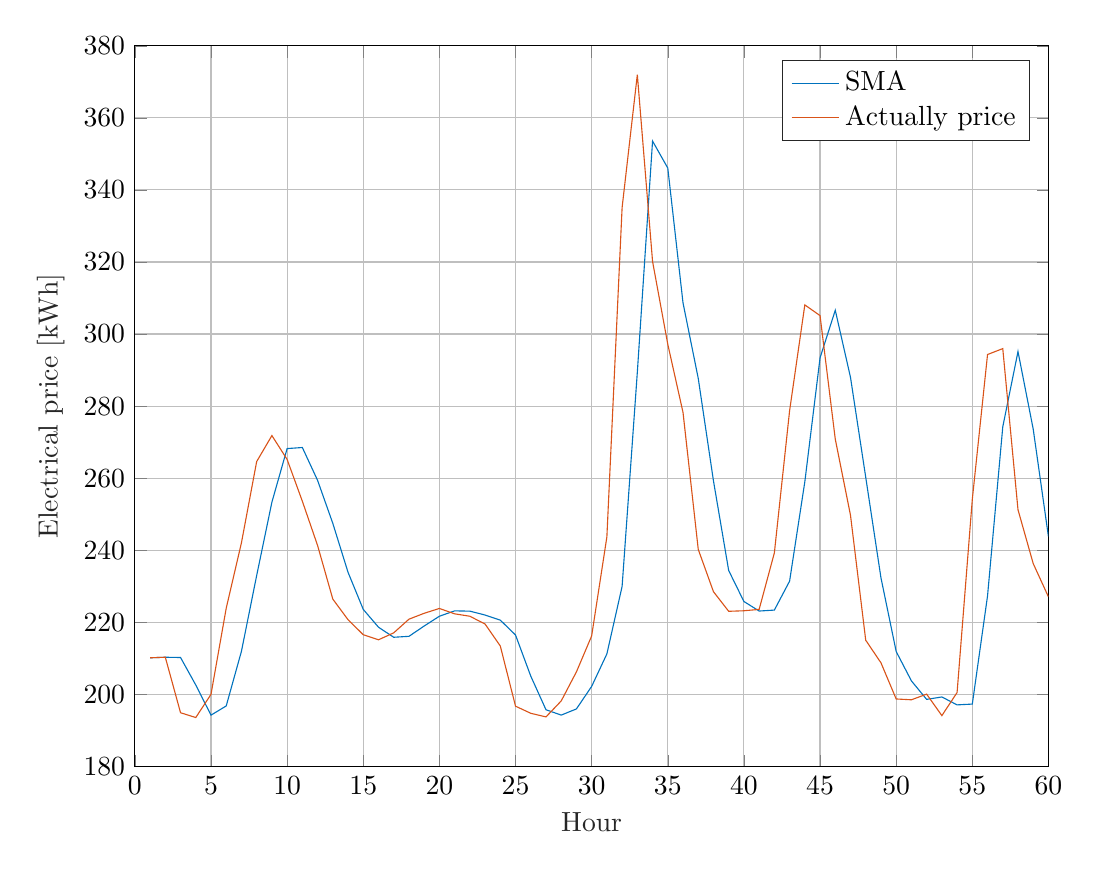
\begin{tikzpicture}

\begin{axis}[%
width=4.568in,
height=3.603in,
at={(0.766in,0.486in)},
scale only axis,
xmin=0,
xmax=60,
xlabel style={font=\color{white!15!black}},
xlabel={Hour},
ymin=180,
ymax=380,
ylabel style={font=\color{white!15!black}},
ylabel={Electrical price [kWh]},
axis background/.style={fill=white},
xmajorgrids,
ymajorgrids,
legend style={legend cell align=left, align=left, draw=white!15!black}
]
\addplot [color=mycolor1]
  table[row sep=crcr]{%
1	210.15\\
2	210.3\\
3	210.225\\
4	202.6\\
5	194.2325\\
6	196.7825\\
7	211.955\\
8	232.99\\
9	253.34\\
10	268.215\\
11	268.51\\
12	259.4\\
13	247.46\\
14	233.88\\
15	223.58\\
16	218.635\\
17	215.845\\
18	216.105\\
19	218.965\\
20	221.68\\
21	223.17\\
22	223.095\\
23	222.015\\
24	220.6\\
25	216.4725\\
26	205.0725\\
27	195.7325\\
28	194.2425\\
29	195.955\\
30	202.205\\
31	211.225\\
32	229.955\\
33	289.4\\
34	353.555\\
35	346.08\\
36	308.655\\
37	287.71\\
38	259.25\\
39	234.365\\
40	225.77\\
41	223.125\\
42	223.39\\
43	231.425\\
44	258.99\\
45	293.4\\
46	306.605\\
47	287.97\\
48	260.255\\
49	232.355\\
50	211.89\\
51	203.74\\
52	198.605\\
53	199.275\\
54	197.08\\
55	197.3\\
56	227.32\\
57	274.23\\
58	295.14\\
59	273.6\\
60	243.765\\
};
\addlegendentry{SMA}

\addplot [color=mycolor2]
  table[row sep=crcr]{%
1	210.15\\
2	210.3\\
3	194.9\\
4	193.565\\
5	200\\
6	223.91\\
7	242.07\\
8	264.61\\
9	271.82\\
10	265.2\\
11	253.6\\
12	241.32\\
13	226.44\\
14	220.72\\
15	216.55\\
16	215.14\\
17	217.07\\
18	220.86\\
19	222.5\\
20	223.84\\
21	222.35\\
22	221.68\\
23	219.52\\
24	213.425\\
25	196.72\\
26	194.745\\
27	193.74\\
28	198.17\\
29	206.24\\
30	216.21\\
31	243.7\\
32	335.1\\
33	372.01\\
34	320.15\\
35	297.16\\
36	278.26\\
37	240.24\\
38	228.49\\
39	223.05\\
40	223.2\\
41	223.58\\
42	239.27\\
43	278.71\\
44	308.09\\
45	305.12\\
46	270.82\\
47	249.69\\
48	215.02\\
49	208.76\\
50	198.72\\
51	198.49\\
52	200.06\\
53	194.1\\
54	200.5\\
55	254.14\\
56	294.32\\
57	295.96\\
58	251.24\\
59	236.29\\
60	227.06\\
};
\addlegendentry{Actually price}

\end{axis}
\end{tikzpicture}%
\caption{Graph of electricity prices from Denmark from the 27-03-2017 to 29-03-2017.}
\label{fig:electrical_price} 
\end{figure}

%The graph seen on \figref{fig:electrical_price}  shows an interval of a 60 hours from the 27-03-2017 to 29-03-2017 in Denmark.
% Even though the pricing seen in \figref{fig:electrical_price} is not a prediction of the future electrical pricing it is assumed to be a good representation of the pricing and therefor it will be used for this project. 

% It can be seen that the SMA is not a precise predictor and have a delay of two hours. However it still keeps the dynamics of the price, which is deemed enough for this project.
